\documentclass[11pt]{article}


\usepackage{geometry}
\usepackage{subcaption} 
\geometry{letterpaper}


\usepackage{doc}
\usepackage{cite}
\usepackage[margin=1cm]{caption}

\usepackage{url}


\usepackage{graphicx}
\usepackage{epstopdf}
\DeclareGraphicsRule{.tif}{png}{.png}{`convert #1 `dirname #1`/`basename #1 .tif`.png}


\title{A ``Dream'' Interface Design}
\author{Rachel Rivera}
\date{November 25, 2014}


\begin{document}


\maketitle


\begin{abstract}
This investigation purposes a ``dream'' user interface for touch screen devices. 
\end{abstract}


\pagebreak
\tableofcontents



\pagebreak


\section{Introduction}
\label{Introduction}

Mobile devices are ubiquitous in contemporary society. The latest figures from the United Nations' telecommunications agency estimate that there are around 6.8 billion cell-phone subscriptions in the world \cite{UNTelecommunications	}. Thus, the investigation and development of usable interfaces for mobile devices is a significant research topic.

Many mobile devices utilize touch screens instead of physical keyboards or buttons. This allows for a larger display without increasing the size of the device. Furthermore, touchscreen keyboards and buttons have the ability to change their layout based on user input and disappear when not needed. To compensate for the lack of tactile feedback provided by physical keys and buttons, touchscreen devices often include aural feedback in the form of audible clicks from a speaker. Haptic feedback in the form of device vibrations is often included as well.

Even with these alternate forms of feedback, the literature suggests that insufficient feedback is still a major usability issue with touchscreen mobile devices. \cite{Tinwala:2010:ETE:18	68914.1868972, Kane:2011:UGB:1978942.1979001, Hardy:2008:TIT:1409240.1409267, El-Glaly:2013:TTF:2460625.2460665, Buxton:1986:HID:22339.22386}. A study by Hussain Tinwala and Scott MacKenzie submits that the lack of physical keys requires heightened visual attention from the user, which diverts the user's concentration from the thoughts being expressed \cite{Tinwala:2010:ETE:18 68914.1868972}. The lack of physical keys not only diverts the attention of some users, but it also makes the device  almost entirely unusable for other users. A study from Virginia Polytechnic Institute and State University demonstrates how touchscreen mobile devices do not provide sufficient feedback for Individuals with Blindness or Severe Visual Impairment (IBSVI) as these users are only able to ``develop a spatial mental model for the interface or the screen through dead reckoning'' \cite{El-Glaly:2013:TTF:2460625.2460665}. 

Thus, the aim of this investigation is to propose a ``dream'' interface design that addresses some of these usability issues.


\section{System Description}
\label{System Description}

In this investigation, I propose a ``dream'' interface design for touchscreen mobile devices that focuses on providing the user with as much as feedback as possible. This feedback is designed in a way that aims to be helpful for users with visual impairments and users without visual impairments alike. The design in its entirety was created with the usability metrics of learnability, efficiency, and error rate in mind.

My ``dream'' interface design incorporates functionality of a product that is currently being developed by Tactus Technology \cite{Tactus}. Tactus Technology, a company based in Fremont, California, creates real physical buttons that dynamically appear and disappear into a flat touch screen (see Figure~\ref{tactus1}). Small fluid channels are routed throughout the Tactile Layer and enable fluid to expand the top polymer layer to create the physical buttons \cite{Tactus}.

Although this technology from Tactus is extremely bleeding-edge, the prototypes have already received a fair amount of recognition as well as several awards \cite{CNN, I-Zone, PCMag, Wired}. Reviewers have articulated how the technology seems to be ``downright magical'' \cite{CNN}. Though the look and feel of Tatctus technology seems totally futuristic, the technology is already beginning to appear in consumer devices. In 2013, Touch Revolution, the largest-volume glass projected capacitive multi-touch screen manufacturer in the world, announced a partnership with Tactus Technology \cite{TactusAvailability}. The technologies are being combined and manufactured into consumer devices today \cite{TactusAvailability}. Not only is this technology becoming more and more available, but it is becoming more customizable as well. Companies will soon be able to customize the panel for different types of buttons, say for example, the buttons on a TV remote \cite{CNN}.

\begin{figure}[ht]
\centering
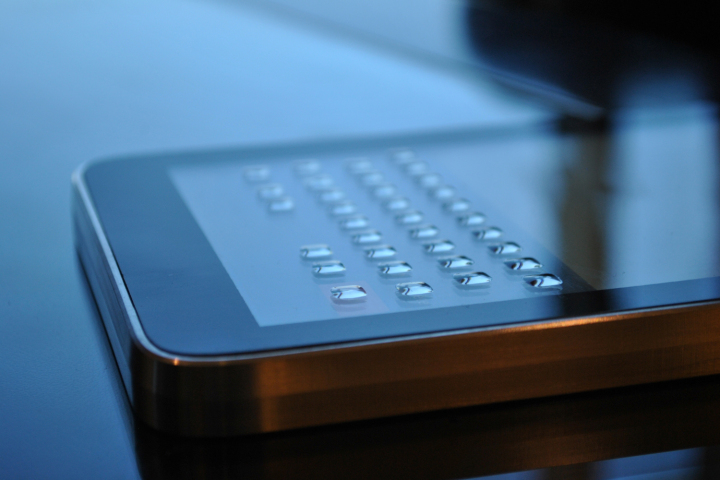
\includegraphics[width=4.5in]{tactus2.jpg} 
\caption{Tactus Technology keyboard}
\label{tactus1}
\end{figure}

My ``dream'' user interface design makes use of the tactile feedback as well as the flexibility that this technology from Tactus provides.


\section{Top-Level Design}
The objective of this ``dream'' interface design is to make mobile touchscreen devices more usable for individuals with visual impairments and individuals without visual impairments alike. The three main features of the design used to attempt to accomplish this goal are the optional physical grid, the tactile buttons, and the auditory feedback. 


\subsection{Optional Physical Grid}
The design incorporates Tactus technology to provide an optional tactile grid for the device (see Figure~\ref{wireframe-grid}). The grid layout would consist of a set of three-dimensional horizontal lines and vertical lines, which could be enabled by the user in the device settings . Both sets of lines are arranged with equal space between each line. The main purpose of this grid is to help IBSVI formulate a mental reference for location awareness to maintain place on the screen.


\begin{figure}[ht]
\centering
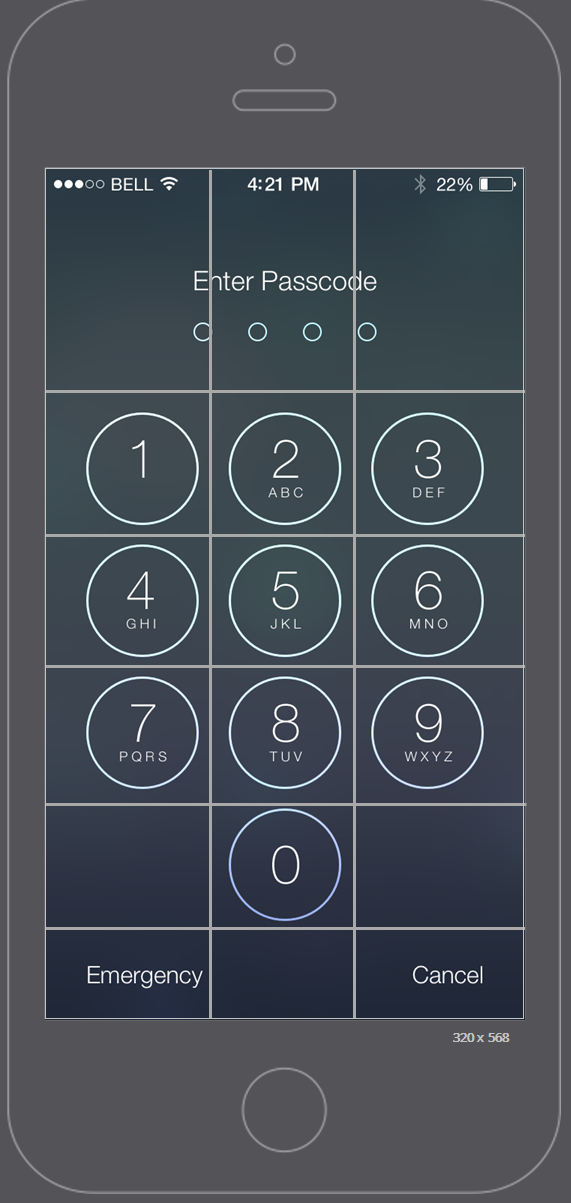
\includegraphics[width=2in]{wireframe-grid.png} 
\caption{A simple wireframe demonstrating the grid layout idea. Each line in the figure would actually be a three-dimensional line that appears on the screen with the use of microfluidic technology from Tactus.}
\label{wireframe-grid}
\end{figure}

\subsection{Tactile Buttons}
The design also includes tactile buttons that rise up and recede as needed (see Figure~\ref{buttons}). This aspect of the design would also be made possible with the use of technology from Tactus. Ideally, the mobile device would be ``intelligent'' about which buttons rose up on the flat screen depending on input from the user.
 
\begin{figure}[ht]
\centering
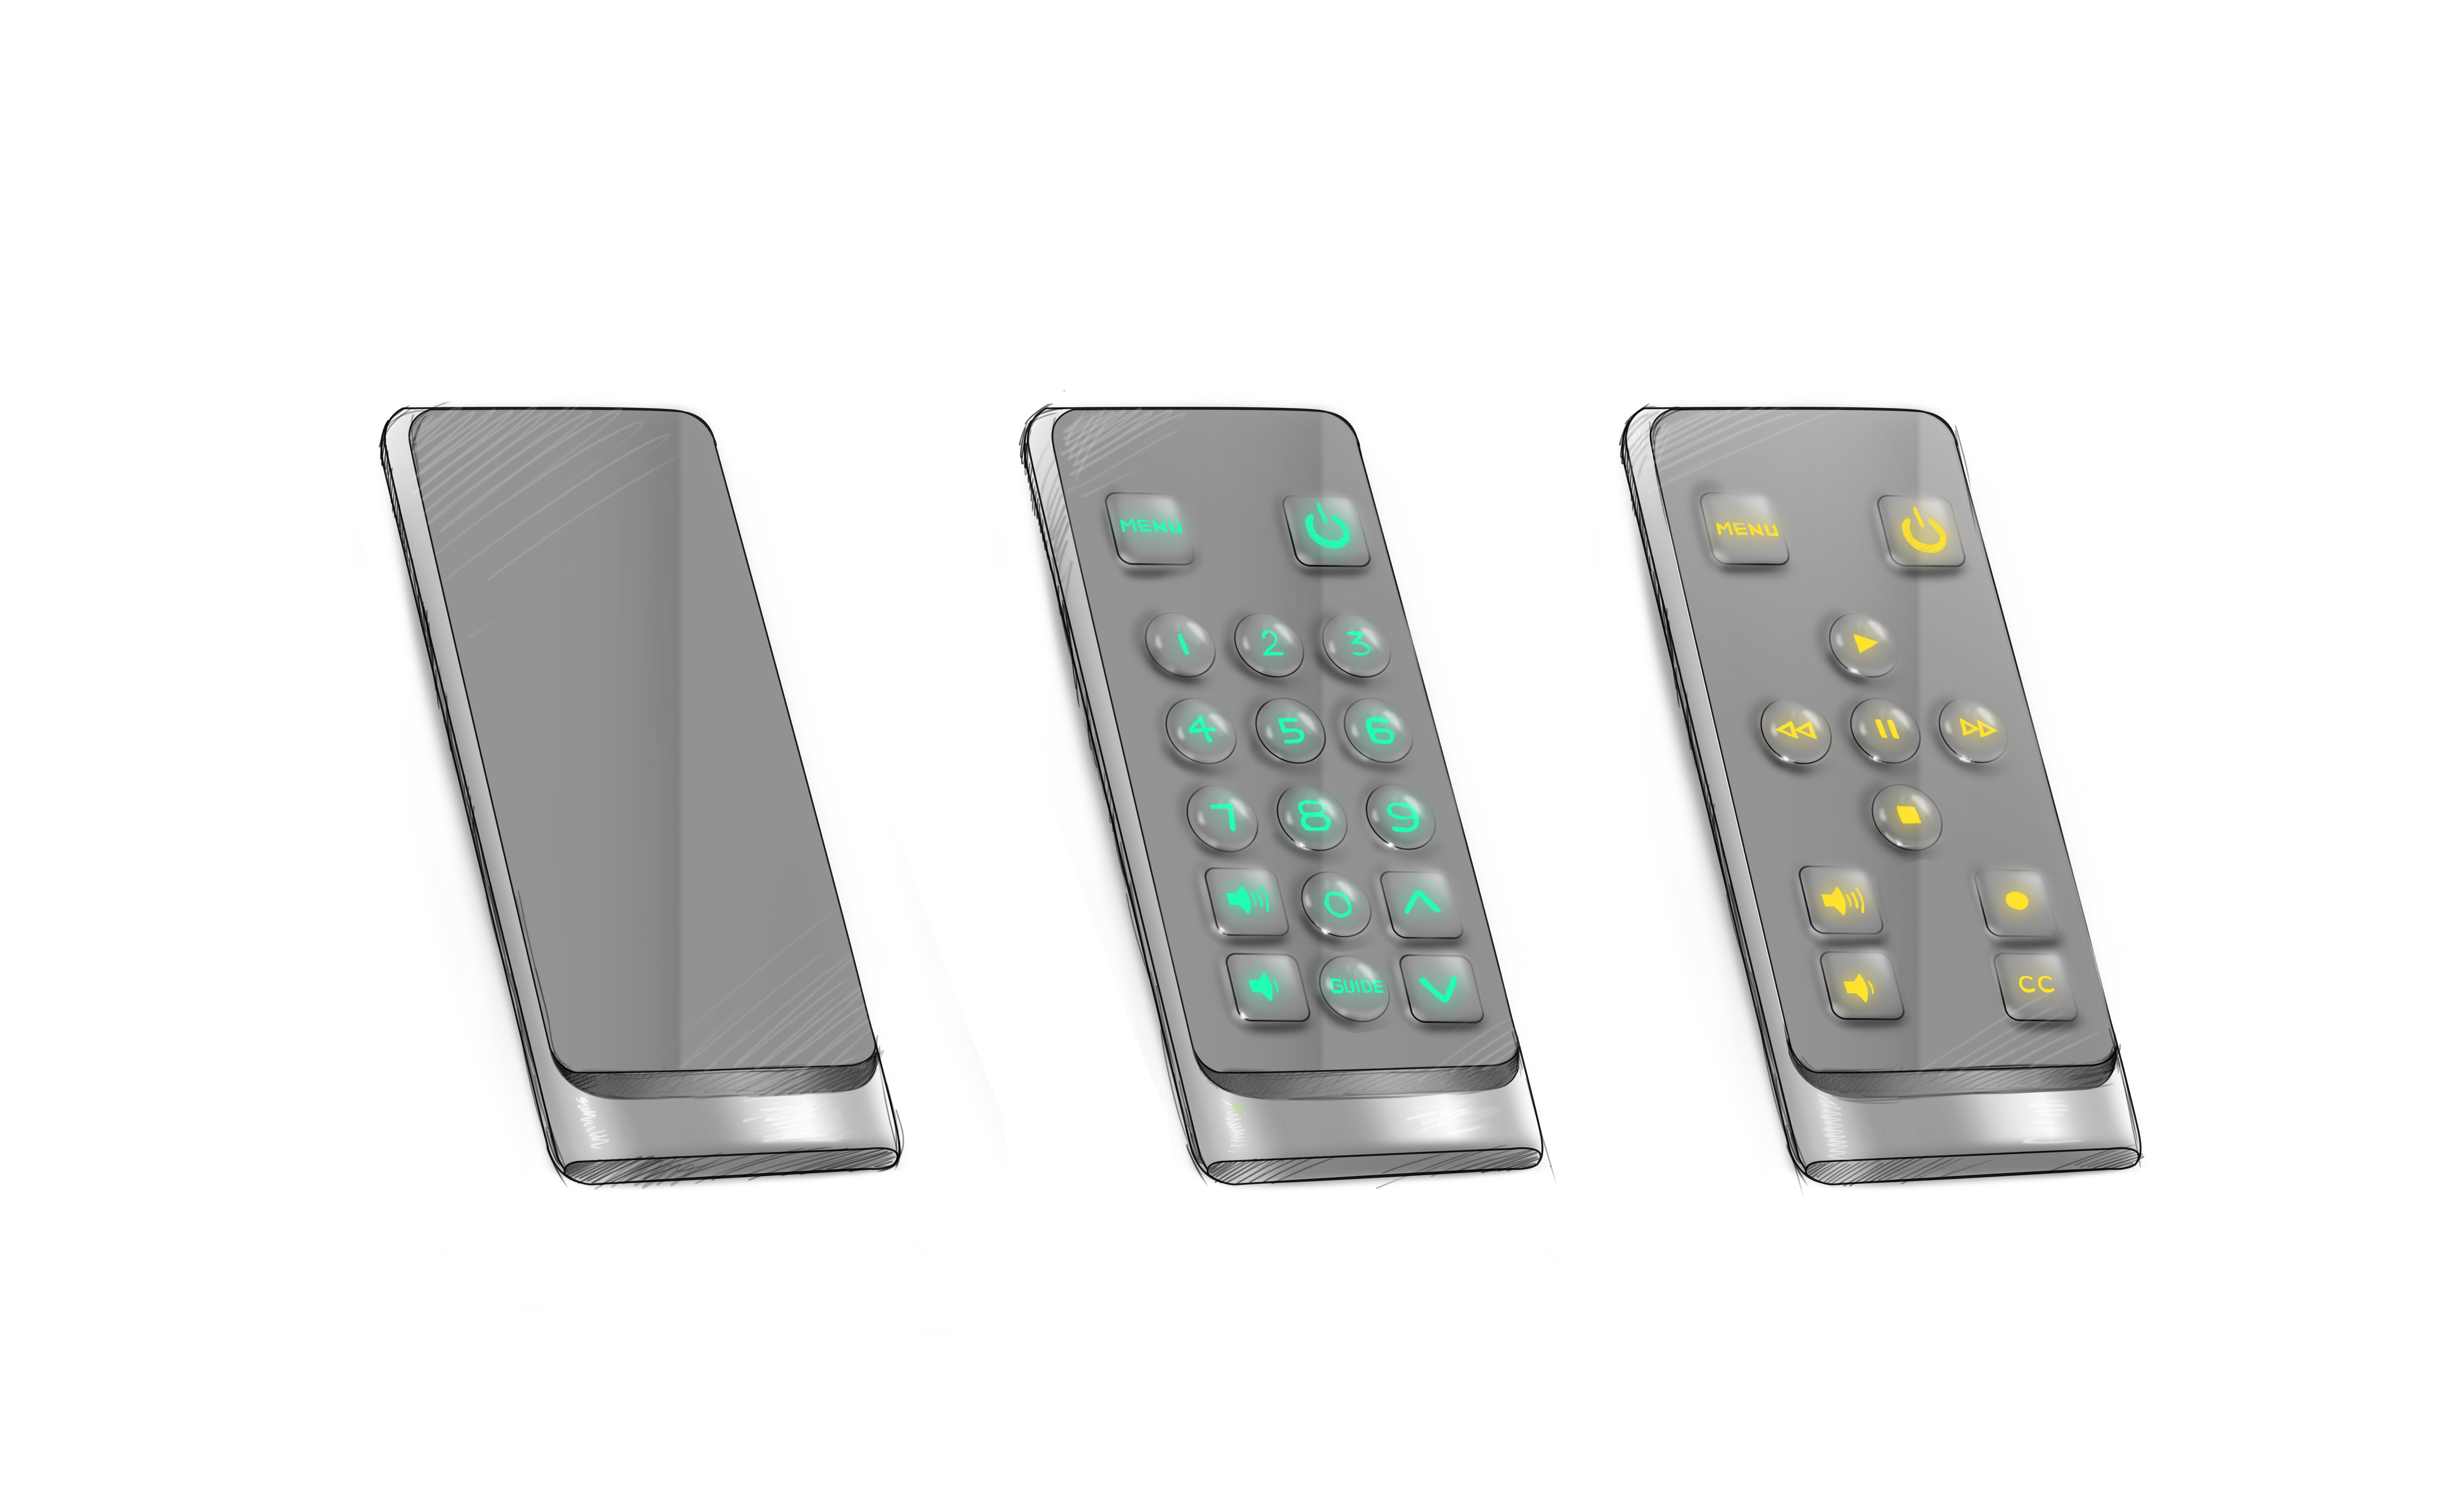
\includegraphics[width=6in]{buttons.jpg}
\caption{A simple representation demonstrating the idea of different subsets of buttons rising up on the same surface at different times.}
\label{buttons}
\end{figure}

In instances when less options are available to the user, less buttons should rise up from the screen. Similarly, when more options are available to the user, more buttons should rise up from the screen. This design aspect should provide more clarity with respect to control flow and what the user is capable of doing at any moment.

\subsection{Auditory Feedback}
The design of this interface was created in such a way that the tactile aspects are intended to operate in conjunction with other technologies that provide auditory feedback. This feedback can inform the user of \textit{what} is at the location on the screen whereas the tactile buttons and grid helps the user know \textit{where} it is.


\section{Usage Scenarios}
There exist several usage scenarios for this interface design. Sighted users employ vision to tell the user what and where to touch, but this interface lacks accessibility for IBSVI because it lacks physical landmarks and tangible buttons. A typical solution is to provide voice over to provide this information, but there is nothing to guide IBSVI to that location in the first place, and there are no landmarks other than dead-reckoning and pure spatial memory to support navigation for the IBSVI. For example, the Apple operating system, iOS, has VoiceOver function, and the Android OS has a Talkbalk function. iOS VoiceOver reads aloud the icon, the user should double tap on that location without the benefit of vision to ensure that the finger does not stray from the touch point. 

The problem with such accessibility modes is that the user can develop a spatial mental model for the interface or screed only through dead reckoning to find VoiceOver locations, in the absence of any landmark other than the boundary of the device. The optional tactile grid as well as the three-dimensional buttons that appear with this design solves this problem. The additional tactile feedback and physical landmarks can guide IBSVI to interact efficiently and effectively with the touch device and its voice over functionality.

Another use case for this interface pertains specifically to the ``intelligent'' tactile buttons. Users often may get overwhelmed by the number of options that are always available to them. It also may be frustrating for users to try to perform a task and not be able to. To examine a specific example, let's say that the user cannot take any more photos on their phone since they are out of memory. In this case, the interface would not even raise the button used to capture photos. This is a good indicator to the user that they need to perform some kind of an action before proceeding.

\section{Rationale}
The tactile stuff is intended to operate in conjunction with other technologies that provide auditory feedback that informs the users of \textit{what} is at the location on the screen while the tactile buttons heps the user know \textit{where} it is. 
The design incorporates Tactus technology to pa physical grid-like layout on the screen. This layout IBSVI so that they can engage their spatial cognition, perception and sensing resources while interacting with touch screens. The design will only enable the grid-like system on-command so to not distract or annoy those who do not benefit from it.

\section{Usability Metric ``Forecast''}
\clearpage


\bibliography{mybib}{}
\bibliographystyle{plain}
\end{document}

\end{document}
	